\documentclass{article}
\usepackage{amsmath,tikz}
\usepackage[margin=3cm]{geometry}
\usetikzlibrary{shapes,arrows,fit}
\title{TinySR}
\author{Peter Schmidt-Nielsen}
% Define block styles
\tikzstyle{block} = [rectangle, draw, fill=blue!20, text width=4.5em, text centered, node distance=2.3cm, minimum height=4em]
\tikzstyle{line} = [draw, -latex']
\tikzstyle{io} = [draw, ellipse,fill=red!20, node distance=3cm, minimum height=2em]
\tikzstyle{config} = [draw, ellipse,fill=green!20, node distance=3cm, minimum height=2em]
\begin{document}
\maketitle
\begin{abstract}
TinySR is a light weight real-time small vocabulary speech recognizer written entirely in portable C.
The entire library fits in a single file (plus header file), and is under a single KLOC.
The primary goal of the project is to provide a clean, well documented teaching implementation of a basic Dynamic Time Warping recognizer.
As a secondary goal, a usable, small footprint recognizer is provided.
The entire project (all the code, training scripts, data and documentation) are released into the public domain, to maximize their pedagogical utility.
This document describes how TinySR works.
\end{abstract}
\section{Overview}
The TinySR processing chain consists of a bunch of steps, summarized in this diagram:
\begin{center}
\makebox[\textwidth]{
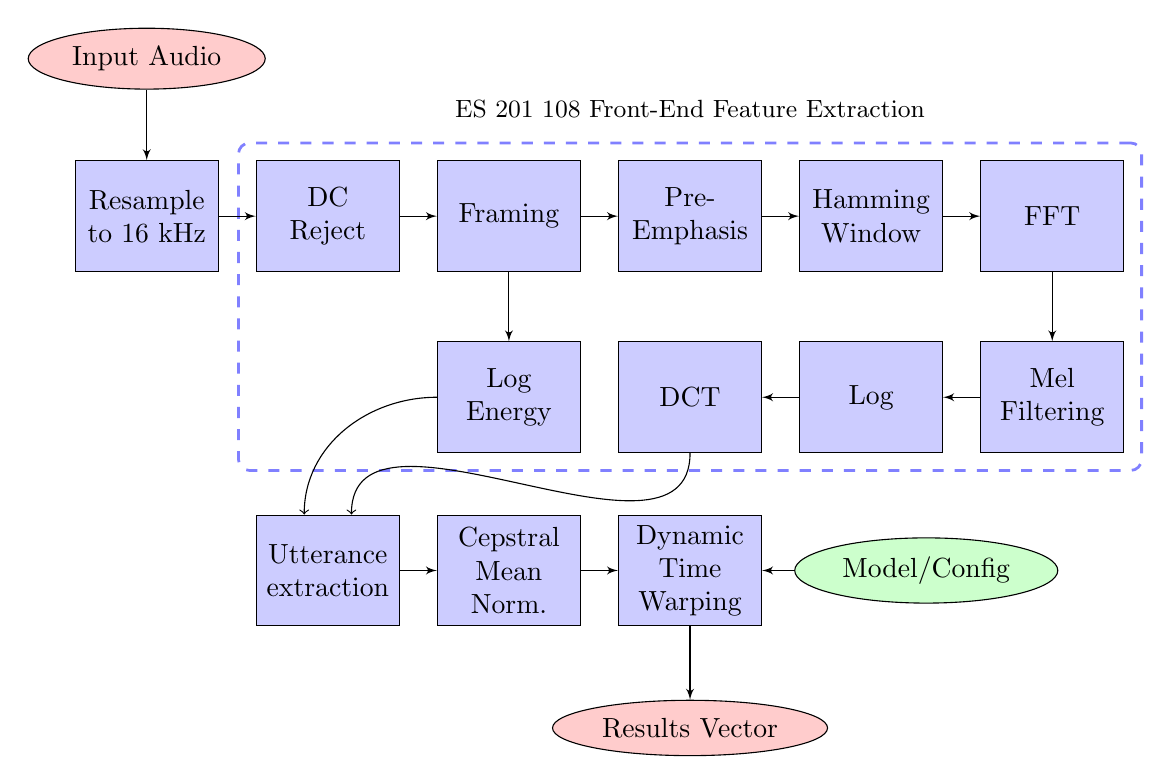
\begin{tikzpicture}[node distance=2cm, auto]
	\tikzset{blue dotted/.style={draw=blue!50!white, line width=1pt, dash pattern=on 4pt off 4pt, inner sep=2.2mm, rectangle, rounded corners}};
	\node [io] (audio) {Input Audio};
	\node [block, below of=audio, node distance=2cm] (resample) {Resample to 16 kHz};
	\node [block, right of=resample] (offset) {DC Reject};
	\node [block, right of=offset] (framing) {Framing};
	\node [block, right of=framing] (pe) {Pre-Emphasis};
	\node [block, right of=pe] (windowing) {Hamming Window};
	\node [block, right of=windowing] (fft) {FFT};
	\node [block, below of=fft] (mel) {Mel Filtering};
	\node [block, left of=mel] (log) {Log};
	\node [block, left of=log] (dct) {DCT};
	\node [block, below of=framing] (loge) {Log Energy};
	\node [blue dotted, fit=(offset) (loge) (mel)] (es201108) {};
	\node at (es201108.north) [above, inner sep=3mm] {\small ES 201 108 Front-End Feature Extraction};
	\node [block, below of=offset, node distance=4.5cm] (utter) {Utterance extraction};
	\node [block, text width=4.5em, right of=utter] (cmn) {Cepstral Mean Norm.};
	\node [block, right of=cmn] (dtw) {Dynamic Time Warping};
	\node [config, right of=dtw] (model) {Model/Config};
	\node [io, below of=dtw, node distance=2cm] (output) {Results Vector};
	\path [line] (audio) -> (resample);
	\path [line] (resample) -> (offset);
	\path [line] (offset) -> (framing);
	\path [line] (framing) -> (pe);
	\path [line] (pe) -> (windowing);
	\path [line] (windowing) -> (fft);
	\path [line] (fft) -> (mel);
	\path [line] (mel) -> (log);
	\path [line] (log) -> (dct);
	\path [line] (framing) -> (loge);
	\draw (dct.south) edge[->,out=270,in=90] ([xshift=3mm]utter.north);
	\draw (loge.west) edge[->,out=180,in=90] ([xshift=-3mm]utter.north);
	\path [line] (utter) -> (cmn);
	\path [line] (cmn) -> (dtw);
	\path [line] (dtw) -> (output);
	\path [line] (model) -> (dtw);
\end{tikzpicture}}
\end{center}

\end{document}
